\begin{figure}
    \centering
    \resizebox{0.6\linewidth}{!}{%
        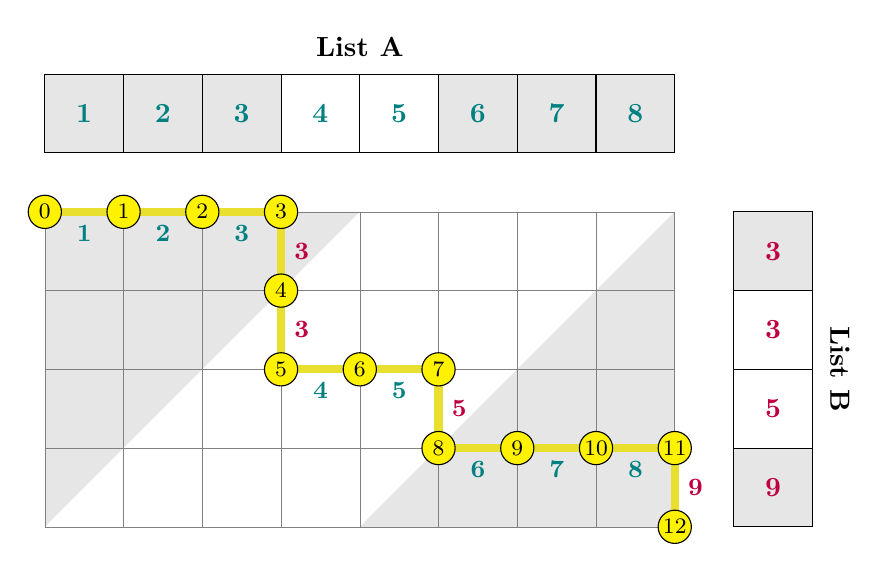
\begin{tikzpicture}
            % Matrix
            \draw[step=1, gray, very thin] (0,0) grid (8,4);

            % List A
            \node[align=center] at (4, 6.1) {\textbf{List A}};
            \draw[fill=gray, fill opacity=0.2] (0, 4.75) rectangle (1, 5.75) node[pos=0.5, teal, fill opacity=1] {\textbf{1}};
            \draw[fill=gray, fill opacity=0.2] (1, 4.75) rectangle (2, 5.75) node[pos=0.5, teal, fill opacity=1] {\textbf{2}};
            \draw[fill=gray, fill opacity=0.2] (2, 4.75) rectangle (3, 5.75) node[pos=0.5, teal, fill opacity=1] {\textbf{3}};
            \draw                              (3, 4.75) rectangle (4, 5.75) node[pos=0.5, teal]                 {\textbf{4}};
            \draw                              (4, 4.75) rectangle (5, 5.75) node[pos=0.5, teal]                 {\textbf{5}};
            \draw[fill=gray, fill opacity=0.2] (5, 4.75) rectangle (6, 5.75) node[pos=0.5, teal, fill opacity=1] {\textbf{6}};
            \draw[fill=gray, fill opacity=0.2] (6, 4.75) rectangle (7, 5.75) node[pos=0.5, teal, fill opacity=1] {\textbf{7}};
            \draw[fill=gray, fill opacity=0.2] (7, 4.75) rectangle (8, 5.75) node[pos=0.5, teal, fill opacity=1] {\textbf{8}};

            % List B
            \node[align=center, rotate=-90] at (10.1, 2) {\textbf{List B}};
            \draw[fill=gray, fill opacity=0.2] (8.75, 0) rectangle (9.75, 1) node[pos=0.5, purple, fill opacity=1] {\textbf{9}};
            \draw                              (8.75, 1) rectangle (9.75, 2) node[pos=0.5, purple]                 {\textbf{5}};
            \draw                              (8.75, 2) rectangle (9.75, 3) node[pos=0.5, purple]                 {\textbf{3}};
            \draw[fill=gray, fill opacity=0.2] (8.75, 3) rectangle (9.75, 4) node[pos=0.5, purple, fill opacity=1] {\textbf{3}};

            % Diagonals + coloring
            \draw[draw opacity=0, fill=gray, fill opacity=0.2] (0, 0) -- (4, 4) -- (0, 4);
            \draw[draw opacity=0, fill=gray, fill opacity=0.2] (4, 0) -- (8, 4) -- (8, 0);

            % Path
            \draw[yellow!80!gray, line width=3pt] (0,4) -- node[below, teal, font=\small]   {\textbf{1}} (1,4);
            \draw[yellow!80!gray, line width=3pt] (1,4) -- node[below, teal, font=\small]   {\textbf{2}} (2,4);
            \draw[yellow!80!gray, line width=3pt] (2,4) -- node[below, teal, font=\small]   {\textbf{3}} (3,4);
            \draw[yellow!80!gray, line width=3pt] (3,4) -- node[right, purple, font=\small] {\textbf{3}} (3,3);
            \draw[yellow!80!gray, line width=3pt] (3,3) -- node[right, purple, font=\small] {\textbf{3}} (3,2);
            \draw[yellow!80!gray, line width=3pt] (3,2) -- node[below, teal, font=\small]   {\textbf{4}} (4,2);
            \draw[yellow!80!gray, line width=3pt] (4,2) -- node[below, teal, font=\small]   {\textbf{5}} (5,2);
            \draw[yellow!80!gray, line width=3pt] (5,2) -- node[right, purple, font=\small] {\textbf{5}} (5,1);
            \draw[yellow!80!gray, line width=3pt] (5,1) -- node[below, teal, font=\small]   {\textbf{6}} (6,1);
            \draw[yellow!80!gray, line width=3pt] (6,1) -- node[below, teal, font=\small]   {\textbf{7}} (7,1);
            \draw[yellow!80!gray, line width=3pt] (7,1) -- node[below, teal, font=\small]   {\textbf{8}} (8,1);
            \draw[yellow!80!gray, line width=3pt] (8,1) -- node[right, purple, font=\small] {\textbf{9}} (8,0);

            % Coordinate nodes
            \draw[fill=yellow] (0,4) circle (6pt) node[font=\footnotesize] {0};
            \draw[fill=yellow] (1,4) circle (6pt) node[font=\footnotesize] {1};
            \draw[fill=yellow] (2,4) circle (6pt) node[font=\footnotesize] {2};
            \draw[fill=yellow] (3,4) circle (6pt) node[font=\footnotesize] {3};
            \draw[fill=yellow] (3,3) circle (6pt) node[font=\footnotesize] {4};
            \draw[fill=yellow] (3,2) circle (6pt) node[font=\footnotesize] {5};
            \draw[fill=yellow] (4,2) circle (6pt) node[font=\footnotesize] {6};
            \draw[fill=yellow] (5,2) circle (6pt) node[font=\footnotesize] {7};
            \draw[fill=yellow] (5,1) circle (6pt) node[font=\footnotesize] {8};
            \draw[fill=yellow] (6,1) circle (6pt) node[font=\footnotesize] {9};
            \draw[fill=yellow] (7,1) circle (6pt) node[font=\footnotesize] {10};
            \draw[fill=yellow] (8,1) circle (6pt) node[font=\footnotesize] {11};
            \draw[fill=yellow] (8,0) circle (6pt) node[font=\footnotesize] {12};
        \end{tikzpicture}
    }
    \caption{Visual representation of parallel merge-sort using three threads\protect\footnotemark.}\label{fig:SPMV-MergePath}
\end{figure}